\section{Completely Randomized Design}

We assume for the moment that the experimental units are homogeneous. We know how to compare two independent groups using the two-sample t-test. If we have more than two groups, this is not applicable anymore.


\subsection{One-Way Analysis of Variance}

On an abstract level we want to compare $g \geq 2$ treatments, having $N$ experimental units, that we assign randomly to the different treatment groups having $n_i$ observations each. This is what we call \textbf{completely randomized design}, it is the most elementary experimental design. If all the treatment groups have the same number of experimental units, we call the design \textbf{balanced}. Such random assignments can be done as follows:

\begin{lstlisting}[language=R]
sample(treat.ord)
\end{lstlisting}

\subsubsection{Cell Means Model}

Let $y_{ij}$ be the observed response from the $j$-th experimental unit in treatment group $i$. In the \textbf{cells mean model} we allow each treatment group (cell) to have its own expected value. This means that $y_{ij}$ is the realised value of the random variable:
$$Y_{ij} \sim \mathcal N(\mu_i, \sigma^2), \; \text{ or } \; Y_{ij} = \mu_i + \epsilon_{ij}, \;\epsilon_{ij} \sim \mathcal N(0, \sigma^2)$$

As for the standard two-sample t-test, the variance is assumed to be equal for all groups. We say that $Y$ is the response and the treatment allocation is a categorical predictor. A categorical predictor is also called a factor. We sometimes distinguish between unordered (or nominal) and ordered (or ordinal) factors. We can rewrite the equation as:
$$\mu_i = \mu + \alpha_i$$

Where $\alpha_i$ is called the \textbf{treatment effect}. This will later help us to untangle the influence of multiple treatment factors on the response. Through this rewrite we have secretly introduced an additional parameter, to remove it again we need a side constraint. Possible constraints could be:

\begin{itemize}
	\item weighted sum-to-zero: $\sum_{i=1}^{g} n_i \alpha_i = 0$
	\item sum-to-zero: $\sum_{i=0}^g a_i = 0$
	\item reference group: $\alpha_1 = 0$
\end{itemize}

For all of the choices it holds that $\mu$ determines some sort of "global level" of the data and $\alpha_i$ contains information about differences between the group means $\mu_i$ from that "global level". If we know $g-1$ of the $\alpha_i$, we automatically know the remaining $\alpha_i$, we also say that the treatment effect has $g-1$ degrees of freedom.

\subsubsection{Parameter Estimation}

We estimate the parameters using the least squares criterion:
$$\hat \mu, \hat \alpha_i = \argmin{\mu, \alpha_i} \sum_{i=1}^g \sum_{j=1}^{n_i}(y_{ij} - \mu - \alpha_i)^2$$

Some notation:
\begin{align*}
	y_{i.} &= \sum_{j=1}^{n_i}y_{ij} 			  \qquad \qquad  \bar y_{i.} = \frac{1}{n_i}y_{i.}\\
	y_{..} &= \sum_{i=1}^g \sum_{j=1}^{n_i}y_{ij} \qquad \ \bar y_{i.} = \frac{1}{N} y_{..}
\end{align*}

As we can independently estimate the values of $\mu_i$, one can show that $\hat \mu_i = \bar y_{i.}$. From $\hat \alpha_i = \hat \mu_i - \hat \mu$ we can get all the other parameters needed (they still depend on the side constraint).

The estimate of the error variance is also called mean squared error $MS_E$:
$$\hat \sigma^2 = MS_E = \frac{1}{N - g} SS_E$$

Where $SS_E$ is the error or residual sum of square:
$$SS_E = \sum_{i=1}^g \sum_{j=1}^{n_i}(y_{ij} - \hat \mu_i)^2$$

\subsubsection{Tests}

With the two-sample t-test, we could test whether two samples share the same mean. We will now extend this for $g > 2$. Saying that all groups share the same mean is equivalent to saying:
$$Y_{ij} = \mu + \epsilon_{ij}, \;\epsilon_{ij} \sim \mathcal N(0, \sigma^2)$$

This is the so-called \textbf{single mean model}, a special case of the cell means model. We have the global null hypothesis
$$H_0 : \mu_1 = ... = \mu_g$$

vs. the alternative hypothesis
$$H_A : \mu_k \neq \mu_l \text{ for at least one pair } k \neq l$$

The idea is to check whether the variation between the different treatment groups (the "signal") is  larger than the variation within the groups (the "noise"). We can decompose the total variation as follows:
$$\underbrace{\sum_{i=1}^g \sum_{j=1}^{n_i}(\bar y_{ij} - \bar y_{..})^2}_{SS_T} = \underbrace{\sum_{i=1}^g \sum_{j=1}^{n_i}(\bar y_{i.} - \bar y_{..})^2}_{SS_{Trt}} + \underbrace{\sum_{i=1}^g \sum_{j=1}^{n_i}(y_{ij} - \hat \mu_i)^2}_{SS_E} $$

All this information can be summarized in a so-called \textbf{ANOVA} table.
\begin{center}
	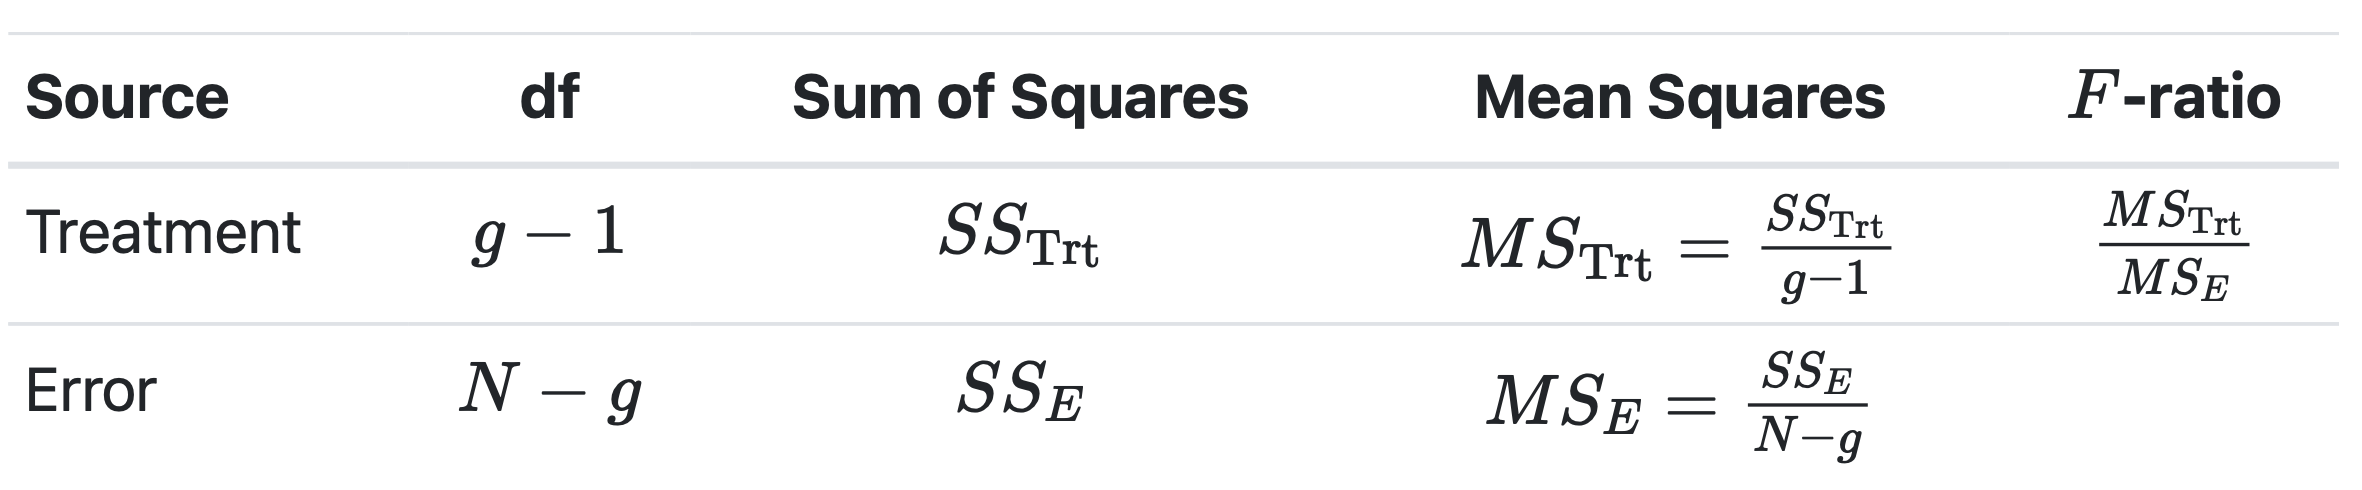
\includegraphics[width=\linewidth]{anova-table.png}
\end{center}

The $MS$ and $SS$ are normalized with the corresponding degrees of freedom. This is a so-called one-way ANOVA, because there is only one factor involved. If all groups share the same expected value, the treatment sum of squares is typically small. We introduce the so called $F$-ratio.
$$F-\text{ratio } = \frac{MS_{Trt}}{MS_E} \sim F_{g-1, N-g}$$

If the variation between groups is substantially larger than the variation within groups (higher F-ratio), we have evidence against the null hypothesis. The $F$-distribution looks as follows:
\begin{center}
	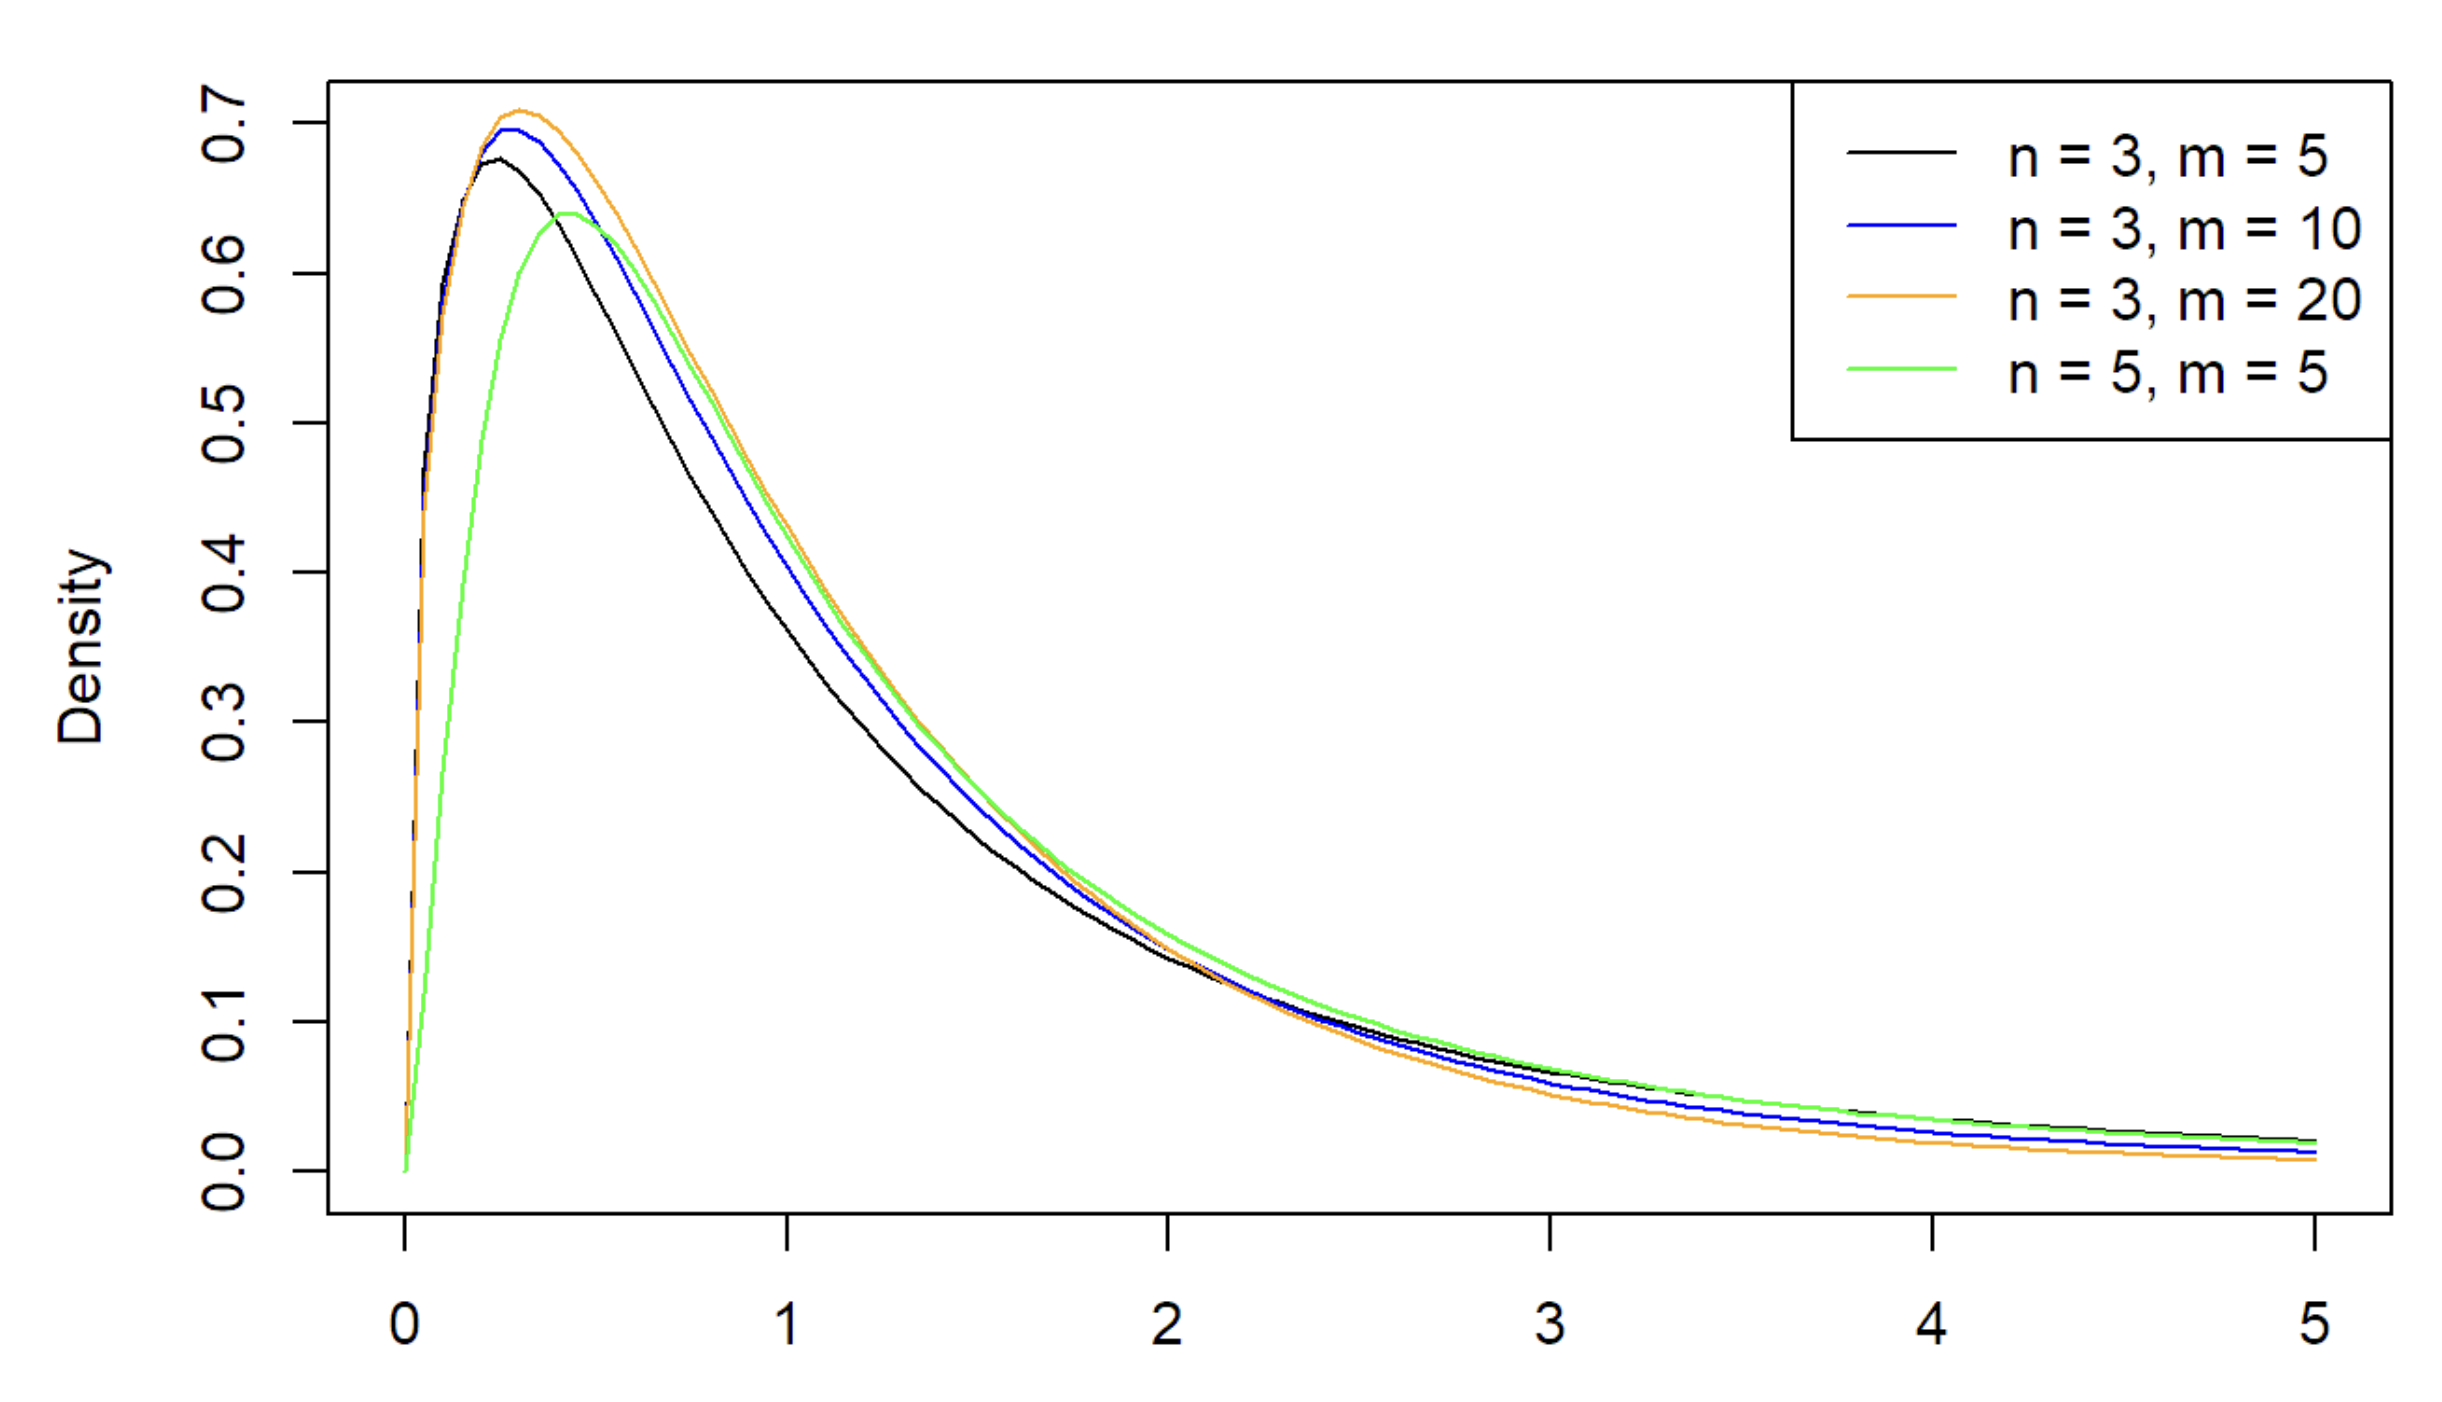
\includegraphics[width=\linewidth]{f-distribution.png}
\end{center}

As with any other statistical test, we reject the null hypothesis if the observed value of the $F$-ratio, our test statistics, lies in an “extreme” region of the corresponding $F$-distribution. As this test is based on the $F$-ratio we call it an \textbf{F-test}.


\subsection{Checking Model Assumptions}

Statistical inference is only valid if all model assumptions are fulfilled. So far this means:
\begin{itemize}
	\item The errors are independent
	\item The errors are normally distributed
	\item The error variance is constant
	\item The errors have mean zero
\end{itemize}

We now introduce different plots to check these assumptions. This means that we use graphical tools to perform qualitative checks.

\subsubsection{QQ-Plot}

In a QQ-plot we plot the empirical quantiles of the residuals or "what we see in the data" vs. the theoretical quantiles or "what we expect from the model". The plot should show a more or less straight line if the normality assumption is correct.
\\[-20pt]
\begin{center}
	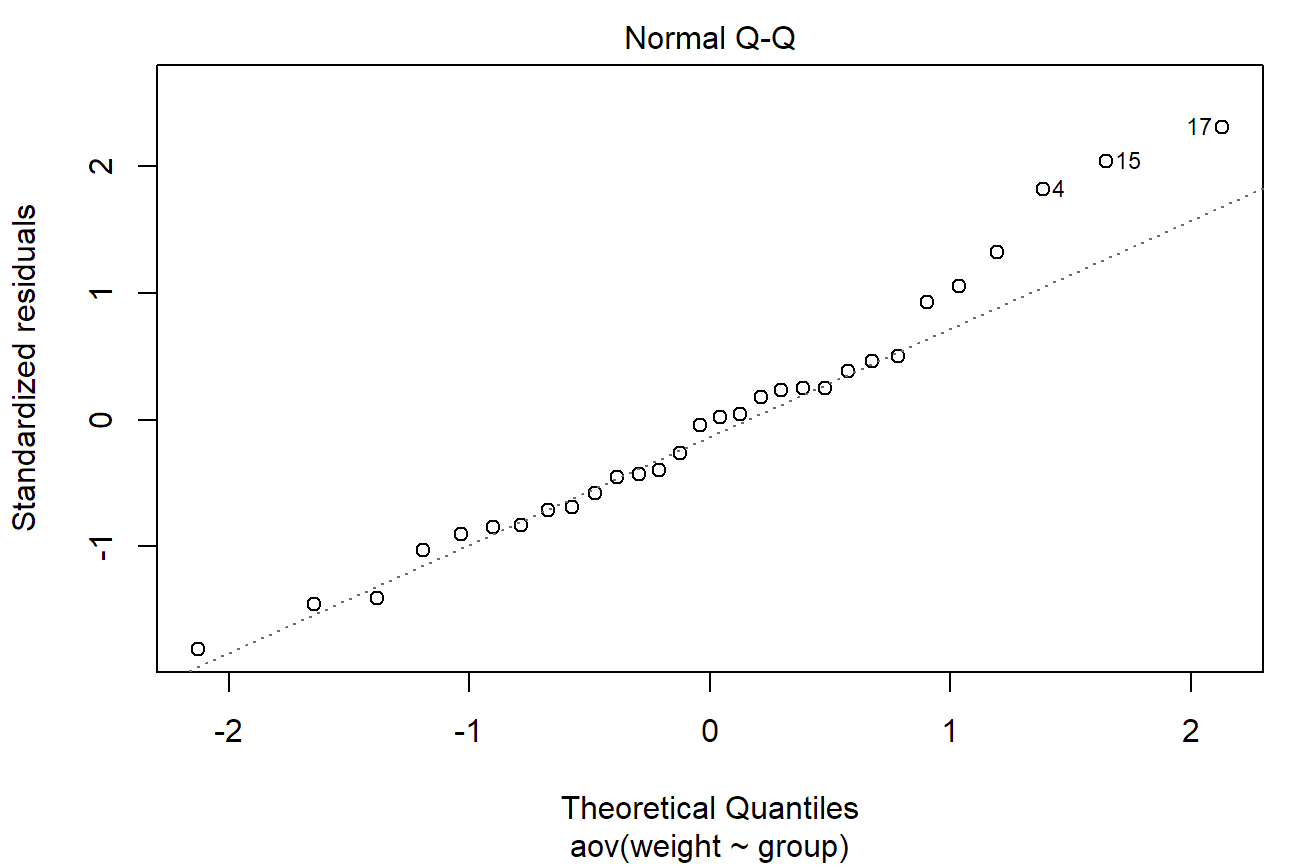
\includegraphics[width=0.9\linewidth]{qq-plot.png}
\end{center}

\subsubsection{Tukey-Anscombe Plot}

The Tukey-Anscombe plot (TA-plot) plots the residuals $r_{ij}$ vs. the fitted values $\hat \mu_i$ (estimated cell means). It allows us to check whether the residuals have constant variance.
\begin{center}
	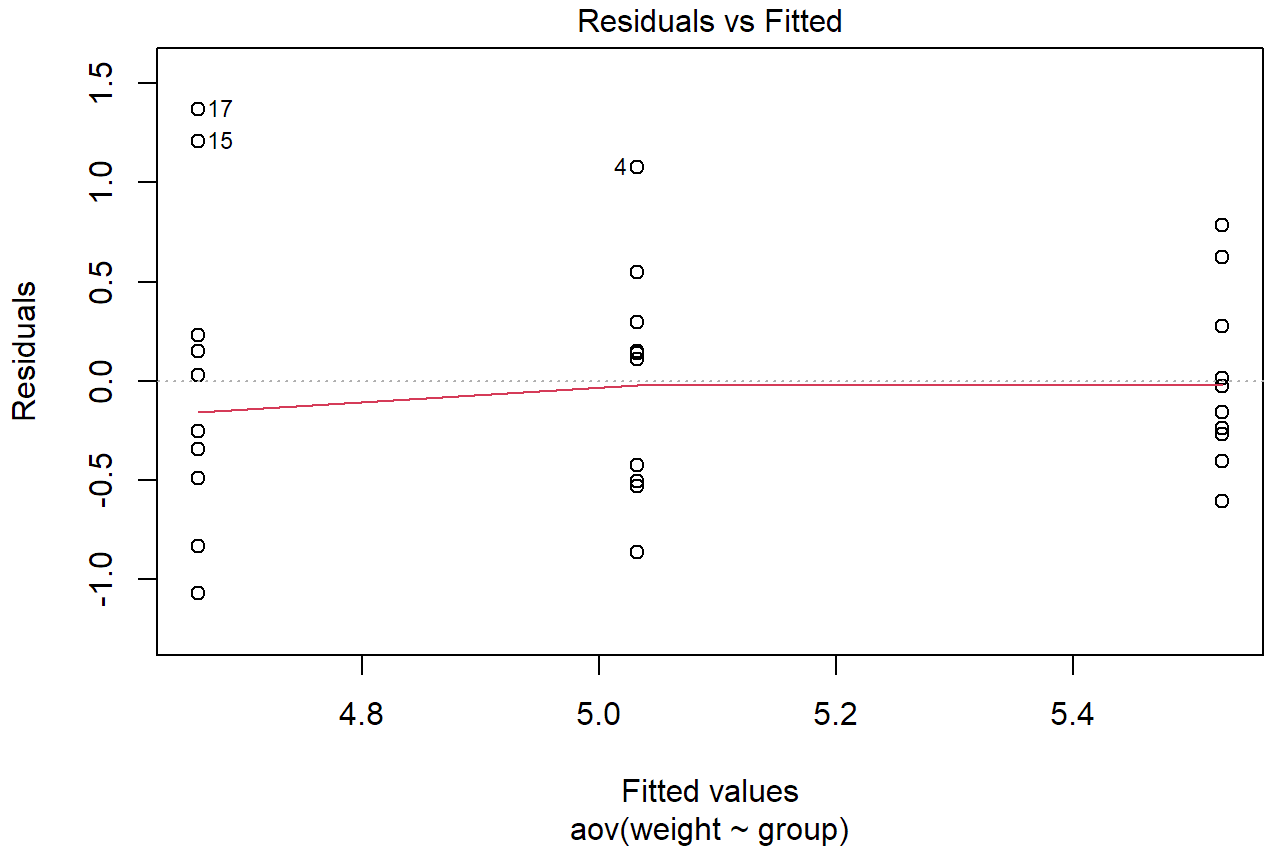
\includegraphics[width=0.9\linewidth]{ta-plot.png}
\end{center}

\subsubsection{Index Plot}

If the data has some serial structure, i.e., if observations were recorded in a certain time order, we typically want to check whether residuals close in time are more similar than residuals far apart. For this we use the index plot where we plot the residuals against time. For positively dependent residuals, we would see time periods where most residuals have the same sign, while for negatively dependent residuals, the residuals would “jump” too often from positive to negative compared to independent residuals. 
\begin{center}
	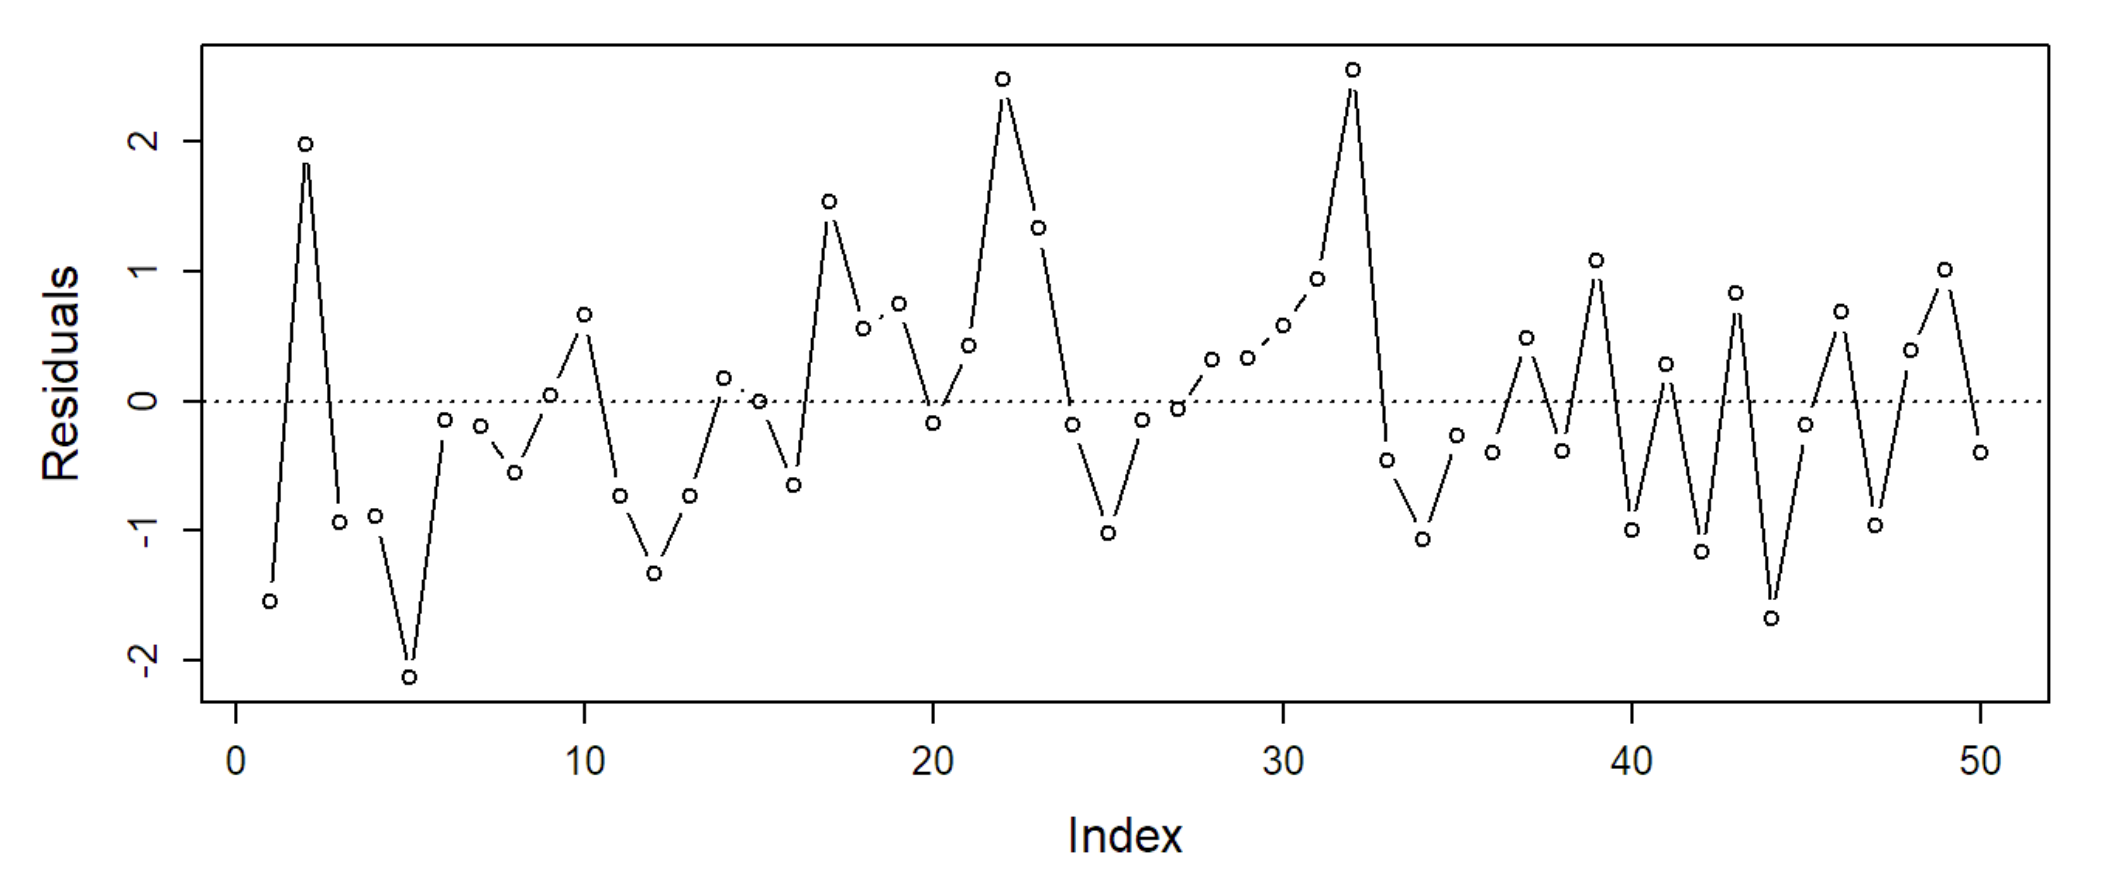
\includegraphics[width=\linewidth]{index-plot.png}
\end{center}


